%\documentclass[twocolumn,showpacs,prb,superscriptaddress,aps,floatfix]{revtex4-1}
\documentclass[preprint,showpacs,prb,superscriptaddress,aps,floatfix]{revtex4-1}
\usepackage{rotating}
\usepackage{amsmath}
\usepackage{color}
\usepackage{graphicx}
\usepackage{epsfig}
\usepackage{courier}
\usepackage[active]{srcltx}
\usepackage[sort&compress]{natbib}


\newcommand{\uu}{{\bf u}}
\newcommand{\qq}{{\bf q}}
\newcommand{\ab}{{\bf a}}
\newcommand{\bb}{{\bf b}}
\newcommand{\hh}{{\bf h}}
\newcommand{\rr}{{\bf r}}
\newcommand{\pp}{{\bf p}}
\newcommand{\PP}{{\bf P}}
\newcommand{\RR}{{\bf R}}
\newcommand{\kk}{{\bf k}}
\newcommand{\HH}{{\bf H}}
\newcommand{\GG}{{\bf G}}
\newcommand{\SiS}{{\bf \Sigma}}
\newcommand{\VV}{{\bf V}}
\newcommand{\UU}{{\bf U}}
\newcommand{\w}{\omega}
\newcommand{\tf}{\textbf}
\newcommand{\bo}{\mathbf}
\newcommand{\br}{{\bf r}}
\newcommand{\be}{\begin{equation}}
\newcommand{\ee}{\end{equation}}
\newcommand{\ben}{\begin{equation*}}
\newcommand{\een}{\end{equation*}}
\newcommand{\bea}{\begin{eqnarray}}
\newcommand{\eea}{\end{eqnarray}}
\newcommand{\bean}{\begin{eqnarray*}}
\newcommand{\eean}{\end{eqnarray*}}
\newcommand{\nup}{n_{\uparrow}}
\newcommand{\ndown}{n_{\downarrow}}
\newcommand{\Id}[1] {\int \! \! {\rm d}^3 #1}
\renewcommand{\v}[1]{{\bf #1}}
\renewcommand{\[}{\left[}
\renewcommand{\]}{\right]}
\renewcommand{\(}{\left(}
\renewcommand{\)}{\right)}
\def\efield{\boldsymbol{\cal E}} 
\def\ket#1{\vert#1\rangle}
\def\bra#1{\langle#1\vert}
\def\pw{^{({\rm W})}}
\def\ph{^{({\rm H})}}
\def\D{{D}\ph}




 
\newcommand{\grenoble}{Institut N\'eel,
CNRS/UJF, 25 rue des Martyrs BP 166, B\^{a}timent D 38042 Grenoble
cedex 9 France} 
\newcommand{\rome}{Istituto di Struttura della Materia (ISM), Consiglio Nazionale delle Ricerche, Via Salaria Km 29.5, CP 10, 00016 Monterotondo Stazione, Italy}
\newcommand{\coimbra}{Centre for Computational Physics and Physics Department, University of Coimbra, Rua Larga, 3004-516 Coimbra, Portugal}

\begin{document}
\title{Simple model for high-harmonic generation}
\author{C. Attaccalite}
\affiliation{\grenoble}

\begin{abstract}
In these notes I consider a simple tight-binding model in Wannier gauge and write down the equation of motion of the density matrix in such a way to study its non-linear response and in particular the high-harmonic generation. I discuss all steps for the implementation in a computational code. 
\end{abstract}           

\maketitle

\section{Unit cell and atomic positions}
As simple system I consider a two-dimensional hexagonal boron nitride as shown in Fig.~\ref{fig:hbn_lattice}. 
\begin{figure}
  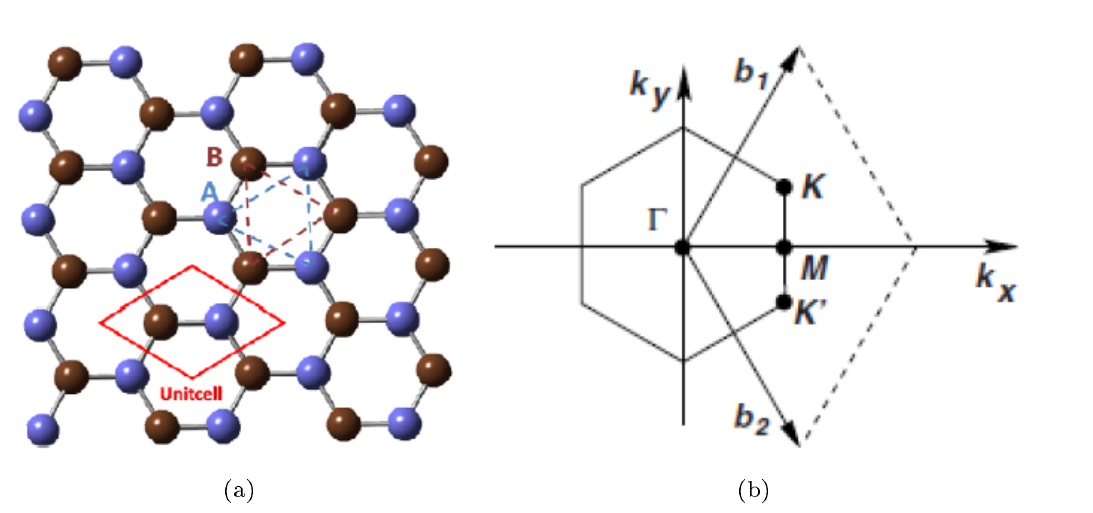
\includegraphics[width=\linewidth]{hbn.png}
  \caption{Hexagonal BN direct and reciprocal lattice.}
  \label{fig:hbn_lattice}
\end{figure}
Lattice vectors are defined as\footnote{I always define quantities in 3D for practical implementation in the code}:
\bea
a_1&=&\frac{a}{2}\left ( 3, \sqrt{3} \right)  \\
a_2&=&\frac{a}{2}\left ( 3, -\sqrt{3} \right)  \\
\eea
and the volume is $V=a_3 \cdot (a_1 \times a_2) = 3\sqrt{3} a^2/2$ 
and reciprocal lattice vectors are defined as:
\bea
b_1&=&\frac{2\pi}{V} a_2 \times a_3 = \frac{2\pi}{a} \left( \frac{1}{3},  \frac{1}{\sqrt{3}}\right) \\
b_2&=&\frac{2\pi}{V} a_3 \times a_1 = \frac{2\pi}{a} \left( \frac{1}{3},  -\frac{1}{\sqrt{3}}\right) \\
\eea

\section{Tight binding model}
As simple model consider a two-band tight-binding model with only the first neighbor hopping, and parameters $t_0=2.92~eV$ and $\epsilon_B = -\epsilon_N = 2.81~eV$. The Hamiltonian reads:
\bea
\tilde H_{11}(\kk)&=&\epsilon_B\\
\tilde H_{22}(\kk)&=&\epsilon_N\\
\tilde H_{21}(\kk)&=&H^*_{12}(\kk) = t_0 \cdot e^{-i \kk_x a}\cdot \left(1+2 \cdot e^{i \kk_x \frac{3 a}{2}} \right)\cdot \cos{ \left( \frac{\sqrt{3} a}{2}\kk_y \right) }
\eea 
Solving these Hamiltonian for each $\kk$ point we get the Bloch wave-function in tight-binding approximation. However we are interested only in the cell-periodic part of the tight-binding wave-functions in such a way to calculate wave-function derivatives and Berry connect.\cite{PythTB} \\
Therefore we define a new Hamiltonian as:
\be
H_{ij}(\kk)=e^{i \kk \cdot (\tau_j -\tau_i) } \tilde H_{ij}(\kk) 
\ee
Or in a matrix notation:
\bea
H(\kk)&=&V^\dagger(\kk) \tilde H(\kk) V(\kk) \\
V_{ij}(\kk)&=& e^{i\kk \tau_i} \delta_{i,j}
\eea
These two Hamiltonians have the same eigenvalues (this is a similarity transformation) but their eigenvectors are related by:
\be
 C_j^{n \kk} = e^{-i \kk \tau_j} \tilde C_j^{n \kk}
\ee
The basis set of the two Hamiltonian are related by:
\bea
|\chi_j^\kk \rangle &=& \sum_\RR e^{i \kk \cdot (\RR + \tau_j)} | \phi_{\RR j} \rangle  \\
|\tilde \chi_j^\kk \rangle &=& \sum_\RR e^{i \kk \cdot \RR } | \phi_{\RR j} \rangle  \\
\eea
and finally Bloch wave-function can be written as:
\bea
|\psi_{n \kk} \rangle &=& \sum_{\RR} \sum_j C_{n \kk}^j e^{i\kk \cdot (\RR + \tau_j) }  | \phi_{\RR j} \rangle \\
|\psi_{n \kk} \rangle &=& \sum_{\RR} \sum_j \tilde C_{n \kk}^j e^{i\kk \cdot \RR  }  | \phi_{\RR j} \rangle
\eea
These results show that $ C_{n \kk}^j$ correspond to the cell periodic solution of the tight-binding and in the literature this choice is called "atomic gauge", while $\tilde C_{n \kk}^j $ contains also the phase factor and it is called "lattice gauge".\cite{wanniertools} These last one is the most common convention in tight-binding but it is not practical for the calculation of Berry phase related objects.
\subsection{Dipoles in "atomic" and "lattice" gauge}
Notice that even if the eigenvalues are the same in the two gauges, the Hamiltonian and the eigenvectors are different. In particular the gradients of the Hamiltonian in Wannier gauge, that used to build dipole are now defined as:
\be
\partial_\alpha \tilde H_{ij}\pw(\kk)=e^{-i \kk \cdot (\tau_j -\tau_i)} \left [ \partial_\alpha H_{ij}\pw + i(\tau_j -\tau_i) H_{ij}\pw(\kk) \right ]
\ee
or in matrix notation
\be
\partial_\alpha \tilde H=V \partial_\alpha H V^\dagger + \partial_\alpha V H V^\dagger +  V H \partial_\alpha V^\dagger 
\ee
the big advantage of this formulation is that now $H_{ij}(\kk)$ is a periodic function of  $\kk$ and its derivatives can be calculated with a standard k-points grid within the first Brillouin zone.\\
For the eigenvectors we use the following relation of the similar matrices. Consider $B=P^{-1}AP \Longleftrightarrow  P B P^{-1} =A$. If $Av=\lambda v$, then $PBP^{-1} v = \lambda v \Longrightarrow BP^{-1} v = \lambda P^{-1} v $. The new eigenvectors of the matrix $B$ are $P^{-1} v$, with the same eigenvalus of $A$.\\
Using the notation $U(\kk)$ for the matrix of the eigenvectors and $V(\kk)$ for the transformation matrix and notice that $V^{-1} = V^{\dagger}$ we can write:
\bea
\partial_\alpha \tilde U &=& \partial_\alpha V^{\dagger} U + V^{\dagger} \partial_\alpha U \\
\tilde U^{\dagger} &=& U^{\dagger} V \\
\tilde U^{\dagger} \partial_\alpha \tilde U &=& U^{\dagger} V \partial_\alpha V^{\dagger} U + U^{\dagger} \partial_\alpha U
\eea
where the term $V \partial_\alpha V^{\dagger}$ is written explicitelly as:
\be
(V \partial_\alpha V^{\dagger})_{nm}=-i\tau_{n,\alpha}\delta_{nm}
\ee
where $\tau_{n,\alpha}$ is the $\alpha$-component of the vector $\tau_n$.

\subsection{Fixing structural gauge in a two band model}
In the previsou section we saw how to get the periodic part of the Bloch function in tight-binding. However in order to calculate Berry connection we have to solve the problem of the structural gauge,\cite{yue2022introduction} namely the problem that due to the numerical diagonalization the wave-function aquires a generic phase factor at each $\kk$ point. We follow the idea of Ref.~\onlinecite{silva2019high} (from a privite discussion), we fix the phase in such a way that the first element of the lowest eigenvectors is real and positive. In this wave, for a system without degenerate state we fix the phase in all the  Brillouin zone.
\section{Wannier and Hamiltonian gauge}
The tight-binding Hamiltonian $H(\kk)$ is a analytic and continuous function of $\kk$, therefore I can define all the derivatives respect to $\kk$ without problems. When we diagonalize $H(\kk)$ on a discrete k-point grid, there is a generic phase attached to the eigenvectors that make complicated the derivative respect to $\kk$. We call Wannier gauge the space before the diagonalization  $H^{W}(\kk)$ and Hamiltonian gauge the space after the diagonalization $H^{H}(\kk)$. Wave-function in the two gauges are related by an unitary transformation:
\begin{equation}
\ket{\psi_{n\boldsymbol{k}}^{\left(H\right)}}=\sum_{m}U_{mn}\left(\boldsymbol{k}\right)\ket{\psi_{m\boldsymbol{k}}^{\left(W\right)}}
\end{equation}
where $U\text{\ensuremath{\left(\boldsymbol{k}\right)}}$ is a unitary
matrix that diagonalizes $H^{(W)}\left(\boldsymbol{k}\right)$,
\begin{equation}
U^{\dagger}\text{\ensuremath{\left(\boldsymbol{k}\right)}}H^{(W)}\left(\boldsymbol{k}\right)U\text{\ensuremath{\left(\boldsymbol{k}\right)}}=H^{(H)}\left(\boldsymbol{k}\right).
\end{equation}
Operators that transforms as the Hamiltonian are called gauge covariant. Operator that contains k-derivative are not gauge covariant and require a more complex transformation.\\
In fact consider the transformation:
\begin{equation}
\ket{u_{n\boldsymbol{k}}^{\left(H\right)}}=\sum_{m}U_{mn}\left(\boldsymbol{k}\right)\ket{u_{m\boldsymbol{k}}^{\left(W\right)}}
	\label{u_transf}
\end{equation}
if we derive respect to $\kk$ we get:
\begin{equation}
	\ket{ \partial_{\kk} u_{n\boldsymbol{k}}^{\left(H\right)}}=\sum_{m}U_{mn}\left(\boldsymbol{k}\right)\ket{\partial_{\kk} u_{m\boldsymbol{k}}^{\left(W\right)}} + \sum_{m}\ket{u_{m\boldsymbol{k}}^{\left(W\right)}} \partial_\kk U_{mn}\left(\boldsymbol{k}\right)
	\label{deriv_u}
\end{equation}
the derivative of quantities in Wannier gauges as $\ket{u_{m\boldsymbol{k}}^{\left(W\right)}}$ are not a problem because they are continuous functions in $\kk$. We can work out the second term using perturbation theory.\cite{wang2006ab} 
Notice that in the perturbation theory we made a gauge choice, and in particular we choose the "parallel transport" gauge see Sec.~$3.7$ in Ref.~\onlinecite{resta}. \\
We consider an Hamiltonian:
\be
H^{(W)} (\kk + \Delta \kk_\alpha) = H^{(W)} (\kk)  + \Delta \kk_\alpha \partial_\alpha  H^{(W)} (\kk)
\ee
where $\partial_\alpha = \partial/\partial_{\kk_\alpha}$. We consider the second term as a perturbation and write the perturbation theory in the Hamiltonian gauge.
\be
	\ket{ u_{n,\boldsymbol{k}+\Delta \kk}^{\left(H\right)}}=\ket{ u_{n,\boldsymbol{k}}^{\left(H\right)}}+\Delta \kk_\alpha \sum_{m} \frac{\bra{u_{m,\boldsymbol{k} }} H^{(W)}_\alpha   \ket{u_{n,\boldsymbol{k} }}}{\epsilon_{m\kk}-\epsilon_{n\kk}} \ket{u_{m,\boldsymbol{k} }}
\ee
where $ H^{(W)}_\alpha =\partial_\alpha  H^{(W)}$. Then we can define the derivative respect to $\kk$ of an eigenvector as:
\be
\ket{ \partial_\alpha u_{n,\boldsymbol{k}}^{\left(H\right)}}=	\frac{\ket{ u_{n,\boldsymbol{k}+\Delta \kk}^{\left(H\right)}}-\ket{ u_{n,\boldsymbol{k}}^{\left(H\right)}}}{\Delta \kk}= \sum_{m \neq n} \frac{\bra{u_{m,\boldsymbol{k} }} H^{(W)}_\alpha   \ket{u_{n,\boldsymbol{k} }}}{\epsilon^{(H)}_{m\kk}-\epsilon^{(H)}_{n\kk}} \ket{u_{m,\boldsymbol{k} }}
\ee
in matrix notation it becomes $ \partial_\alpha U_{mn} = \sum_l U_{ml} D^{(H)}_{ln\alpha}$ and
\begin{equation}
\D_{nm,\alpha}\equiv (U^{\dagger}
\partial_{\alpha}U)_{nm}=
\begin{cases}
  \displaystyle
  \frac{\overline H_{nm,\alpha}^{(\rm H)}}{{\cal E}^{(\rm H)}_{m}
  -{\cal E}_{n}^{(\rm H)}}& \text{if $n\not= m$}\\ \\
  0& \text{if $n=m$}
\end{cases}
\label{eq:ddef}
\end{equation}
If we insert this result in Eq.~\ref{deriv_u} and together with Eq.~\ref{u_transf} we get:
\begin{equation}
	\ket{ \partial_{\kk} u_{n\boldsymbol{k}}^{\left(H\right)}}=\sum_{m}U_{mn}\left(\boldsymbol{k}\right)\ket{\partial_{\kk} u_{m\boldsymbol{k}}^{\left(W\right)}} + \sum_{m}\ket{u_{m\boldsymbol{k}}\ph} \D_{mn,\alpha}
	\label{deriv_uh}
\end{equation}
we will use this result to define the position operator.\\
Notice that rotation from Wannier to Hamiltonian base is equaivalent to take the braket in the Hamiltonian basis. In fact we have that
\bea
\nabla H^H_{ij} = \langle u_{i\kk} | \nabla   H^W | u_{j,\kk} \rangle
\eea
or in the linear algebra notation
\bea
\nabla H^H_{ij} = u^{+}_{i\kk} [ \nabla   H^W ]  u_{j,\kk}
\eea
and then in matrix notation
\bea
\nabla H^H = U^{+}(\kk) [ \nabla   H^W ]  U(\kk)
\eea


\section{Position operator in periodic system}
The position operator in periodic system is defined as:\cite{blount1962solid}
\be
\hat \rr = i \frac{\partial}{\partial \kk} + \hat A
\label{rperiodic}
\ee
where $\hat A$ is the transition dipole moment or a generalization of the Berry connection:\cite{silva2019high,wang2006ab}. This operator is well defined in the Wannier gauge.
\be
\boldsymbol{A}\pw_{nm}\left(\boldsymbol{k}\right)=i\int_{V_{C}}d\boldsymbol{r}~u^{*}_{n\boldsymbol{k}}\left(\boldsymbol{r}\right)\frac{\partial}{\partial\boldsymbol{k}}u_{m\boldsymbol{k}}\left(\boldsymbol{r}\right).
\ee
Notice that the presence of the k-derivative in Eq.~\ref{rperiodic} generate an additional term when we rotate it in the Hamiltonian gauge. Using Eq.~\ref{deriv_uh} this term can be rewritten the Hamiltonian gauge as:
\begin{equation}
\boldsymbol{A}^{\left(H\right)}\left(\boldsymbol{k}\right)=U^{\dagger}\text{\ensuremath{\left(\boldsymbol{k}\right)}}\boldsymbol{A}^{\left(W\right)}\left(\boldsymbol{k}\right)U\text{\ensuremath{\left(\boldsymbol{k}\right)}}+iU^{\dagger}\text{\ensuremath{\left(\boldsymbol{k}\right)}}\frac{\partial}{\partial\boldsymbol{k}}U\left(\boldsymbol{k}\right).
\end{equation}
The term $(U^{\dagger}\partial_{\alpha}U)_{nm}$ can be calculated using perturbation theory as deriving directly the eigenvectors if the phase has been fixed. For example in Ref.~\onlinecite{silva2019high} they fix the phase of the eigenvectors by rotating U such that the diagonal of U is real and positive. Notice the this procedure works only if you do not have degenerate states as in their work.\\
The other therm $\boldsymbol{A}^{\left(W\right)}$ can be calculated in different ways: 
\begin{itemize}
\item
Using matrix elements of the position operator in a Wannier basis:
\be
\boldsymbol{A}_{nm}^{(W)}\left(\boldsymbol{k}\right)  \equiv\sum_{\boldsymbol{R}}e^{i\boldsymbol{k}.\boldsymbol{R}}\left\langle \boldsymbol{0}n\left|\hat{\boldsymbol{r}}\right|\boldsymbol{R}m\right\rangle .\label{eq:Berry_connection_Wannier}
\ee
\item In tight-binding using the approximation:\cite{silva2019high}
\be
		\left\langle \boldsymbol{0}n\left|\hat{\boldsymbol{r}}\right|\boldsymbol{R}m\right\rangle=\delta_{nm}\delta_{\boldsymbol{0} \boldsymbol{R}} = \tau_n
\ee
where $\tau_n$ is the center of the n-Wannier function.
\item 
	From the overlaps of the eigenfunctions:\cite{wang2006ab}
	\begin{equation}
        A_{nm,\alpha}\pw(\kk)\simeq
        i\sum_\bb\,
        w_b b_{\alpha}\Big ( \langle u_{n\kk}\pw|u_{m,\kk+\bb}\pw
        \rangle
        - \delta_{nm}\Big )\;,
\label{eq:A_dis}
\end{equation}
%
where $\bb$ are the vectors connecting $\kk$ to its nearest
		neighbors on the {\it ab-initio} mesh, and $w_b$ are the coefficients for the finite difference derivatives. The overlaps in the Wannier gauge can be calculated starting from the ones in the Hamiltonian gauge. We define $S\pw_{nm}(\kk;\kk+\bb) =  \langle u_{n\kk}\pw|u_{m,\kk+\bb}\pw \rangle$ and $S\ph_{ij}(\kk;\kk+\bb) =  \langle u_{i\kk}\ph|u_{j,\kk+\bb}\ph \rangle$. Using Eq.~\ref{u_transf} and its inverse we can write down the transformation between the two overlap matrices as:
\be
		S\pw(\kk;\kk+\bb) = U(\kk) S\ph(\kk;\kk+\bb) U^\dagger(\kk+\bb)
\ee
 
Finally the term  $i {\partial}/{\partial \kk}$ can be calculated directly as a finite difference k-point mesh of the density matrix in the Wannier gauge.
\end{itemize}

\section{Equation of motion}
Using the definition Eq.\ref{rperiodic} for the position operator, it is possible to write down the equation of motion(EOM) for the density matrix in the Wannier gauge as:
\begin{align}
i\hbar\frac{\partial}{\partial t}\rho\pw_{nm}\left(\boldsymbol{k},t\right) & =\left[H\pw\left(\boldsymbol{k}\right),\rho\pw\left(\boldsymbol{k},t\right)\right]_{nm}\nonumber \\
 & +i\left|e\right|\boldsymbol{E}\left(t\right).\frac{\partial}{\partial\boldsymbol{k}}\rho\pw_{nm}\left(\boldsymbol{k},t\right)\nonumber \\
 & +\left|e\right|\boldsymbol{E}\left(t\right).\left[\boldsymbol{A}\pw\left(\boldsymbol{k}\right),\rho\pw\left(\boldsymbol{k},t\right)\right]_{nm}\label{eq:RDM_eq_motion}
\end{align}
Notice that in this gauge everything is smooth function of $\kk$. Then we can rotate these equations in the Hamiltonian gauge, using the relations:
\begin{align}
\rho_{nm}^{\left(H\right)}\left(\boldsymbol{k},t\right) & =\sum_{ab}U_{nb}^{\dagger}\left(\boldsymbol{k}\right)\rho_{ba}^{\left(W\right)}\left(\boldsymbol{k},t\right)U_{am}\left(\boldsymbol{k}\right)\\
	\rho_{nm}^{\left(W\right)}\left(\boldsymbol{k},t\right) & =\sum_{ab}U_{nb}\left(\boldsymbol{k}\right)\rho_{ba}^{\left(H\right)}\left(\boldsymbol{k},t\right)U_{am}^{\dagger}\left(\boldsymbol{k}\right). \label{eq_rho_w}
\end{align}
and we get:
\begin{align}
i\hbar\frac{\partial}{\partial t}\rho_{nm}^{\left(H\right)}\left(\boldsymbol{k},t\right) & =\left[H^{\left(H\right)}\left(\boldsymbol{k}\right),\rho^{\left(H\right)}\left(\boldsymbol{k},t\right)\right]_{nm}\nonumber \\
 & +i\left|e\right|\boldsymbol{E}\left(t\right).\frac{\partial}{\partial\boldsymbol{k}}\rho_{nm}^{\left(H\right)}\left(\boldsymbol{k},t\right)\nonumber \\
	& +\left|e\right|\boldsymbol{E}\left(t\right).\left[\boldsymbol{A}^{\left(H\right)}\left(\boldsymbol{k}\right),\rho^{\left(H\right)}\left(\boldsymbol{k},t\right)\right]_{nm} \label{eq_rho_h}
\end{align}
Notice that in this gauge $A\ph(\kk)$ is composed of two terms, the rotation of $A\pw(\kk)$ and a term that is generated by the derivative in $\kk$ applied to the rotation matrices. Eq.~\ref{eq_rho_h} is obtained from Eq.~\ref{eq_rho_w}, using Eqs.~\ref{eq:RDM_eq_motion} and the fact that $(\partial_\kk  U^\dagger) U = - U^\dagger( \partial_\kk U) $.\\
Notice that in the Hamiltonian gauge we can safely include dephasing or self-energies.
\section{Current and polarization}	
The current is written as:
The matrix representation of the current operator in a Bloch basis
is defined as
\begin{align}
\hat{\boldsymbol{J}} & =\frac{-\left|e\right|}{i\hbar}\left[\hat{\boldsymbol{r}},\hat{H}\left(t\right)\right]\\
\left(\hat{\boldsymbol{J}}\right)_{\boldsymbol{k},nm} & =\frac{-\left|e\right|}{\hbar}\left(\frac{\partial}{\partial\boldsymbol{k}}H_{nm}\left(\boldsymbol{k}\right)-i\left[\boldsymbol{A}\left(\boldsymbol{k}\right),H\left(\boldsymbol{k}\right)\right]_{nm}\right).
\end{align}
In the Hamiltonian gauge, we can identify the two terms in the expression
for the current as the \emph{intraband }and \emph{interband }current.
\begin{align}
\left(\hat{\boldsymbol{J}}_{intra}\right)_{\boldsymbol{k},nm} & =\frac{-\left|e\right|}{\hbar}\left(\frac{\partial}{\partial\boldsymbol{k}}H_{nm}^{\left(H\right)}\left(\boldsymbol{k}\right)\right)\\
\left(\hat{\boldsymbol{J}}_{inter}\right)_{\boldsymbol{k},nm} & =\frac{i\left|e\right|}{\hbar}\left(\left[\boldsymbol{A}^{\left(H\right)}\left(\boldsymbol{k}\right),H^{\left(H\right)}\left(\boldsymbol{k}\right)\right]_{nm}\right).
\end{align}
Notice that the current include the gradient in $\kk$ of $H$ that should be correct from the lattice to the atomic gauge.

\appendix
\section{Derivatives in k-space}
In general to perform derivative in k-space we define quantities as:
\be
\PP = \frac{1}{2\pi} \sum_{i=1,3} \ab_i (\PP \cdot \bb_i) = \frac{1}{2\pi} \sum_{i=1,3} \ab_i \PP_i
\ee
where $\bb_i$ are reciprocal lattice vectors and $\ab_i$ direct lattice vectors that satisfy the relation:
\be
\ab_i \cdot \bb_j = 2\pi\delta_{ij}
\ee
then the derivative along a $\bb_i$ vector can be rewritten in Cartesian coordinates as:
\be
\nabla \PP = \frac{1}{2\pi} \sum_{i=1,3} \ab_i \left( \frac{\partial \PP_i}{\partial \kk_i} |\bb_i| \right)
\ee 
where $\partial \PP_i/\partial \kk_i$ is the derivative along the $\bb_i$ direction, or one can write the finite difference derivative using $\Delta \kk_i = \bb_i/N_i$.
\be
\nabla \PP = \frac{1}{2\pi} \sum_{i=1,3} \ab_i \left( \frac{\Delta \PP_i}{\Delta \kk_i}  |\bb_i|  \right) = \frac{1}{2\pi} \sum_{i=1,3} \ab_i \left( N_i \Delta \PP_i \right)
\ee 

\addcontentsline{toc}{chapter}{Bibliography}
\bibliographystyle{apsrev4-1}
\bibliography{hhg}
\end{document}
